%!TEX root = dissertation.tex

\chapter*{About this project}
\paragraph{Abstract}

Dúchas Na Gaillimhe ( Galway Civic Trust ) along with Tourism Ireland carry out walking tours of Galway city to inform visitors of Galway's long and rich history. One of the walks they offer tourists during the summer months is a medieval walking tour of Galway city. This walk visits seven locations starting in Galways Latin Quarter. However, this limits visitors to attending guide-lead tours at specific times as well as only being available frequently during the summer tourist season.

This project aims to deliver a solution which helps tourists visiting Galway city to take the medieval walking tour of Galway at any time, without the need of a guide and will be available at any time of the year. If the tourist wishes to seek further information they can drop into Galway Civic Trust's office which is located at one of the seven stops along the route - at the Hall Of the Red Earl.

The proposed solution will comprise a mobile phone application which will allow users to be guided around Galway city. It will show the user their current location and guide them to the destination they wish to reach. On arrival at the destination, the app provides the user with information and images about the location. A user can get additional information if they so wish. There will also be a web application used by Galway Civic Trust personnel to update the information on the application periodically and make it automatically available to all new and existing app users.

\paragraph{Authors}
Sarah Carroll, Abigail Culkin
B.Sc.(Hons) in Software Development

\chapter{Introduction}

At the beginning of Year 4 in Software Development at GMIT, the authors were given the opportunity to work on the Medieval walking tour project for an external small/medium Enterprise organised through GMIT. The idea of the project is based on the problem that medieval walking tours of Galway city are not always available for tourists at convienient times and infrequently outside the main summer season. 


The purpose of this Final Year Project is to build an application using new technologies that the developers have never used before. Therefore, it allows for research to be done and learn up and coming technologies and learn new ways of developing software. The front-end technology being used is Flutter. It will be connected to a backend server running on Google cloud platform and within this a MongoDB Flask Database which uses docker. Working with Galway Civic trust allowed for an application to be made that is missing from the market place for Galway tourism. This application will be useful and easy to use for customers and the company will benefit from this.  This way the authors will be able to show they have worked with an outside source and have a fully functioning app that will satisfy what was asked of them.


It will be explained the technologies used and why we used them throughout. The research and development will all be detailed and allow others to understand why specific software was chosen. This project is done using technologies that have not been used together too often. This means any problems faced or certain aspects found to be new will be documented along with the development.
\section{Context}

\subsection{Context of the Project}

The context of this project revolves around the use case of being a tourist in Galway city, wishing to find out more information about the city's history. Opening the app on your phone, viewing your location in relation to the locations on the guided tour. This application prevents the user getting lost and gives them accurate information about each location.  The information on the application was provided by Galway Civic Trust and is the same information a tourist gets on the guided walking tours. Reading the data and retrieving images from the database needs to be very fast, as any delayed hang in performance could lead to a bad user experience.

The project will be developed as a Cross-Platform application which provides users with images, information and a map of Galway city and the seven medieval stops along the tour. Users of the application can get their location in relation to the exact location of the points of the tour at any given time. When the user decides they wish to learn more information about a specific location, the user can retrieve images and text about the location on the application. Along with the  mobile application a web application will be developed for use by Galway Civic Trust personnel to update, delete or add information to the tour database.

\section{Objectives} 


The project will require a number of objectives to be accomplished in order to provide a solution that works and is suitable for the use of Galway Civic Trust. 

\begin{itemize}
\item A Mongo database will be used to store the text and images which appear in the application. This database will need to be setup and hosted in such a way that it can be accessed from clients on the web. The database will be hosted on Amazon Web Services Cloud.

\item A client application will be the main product / asset for the project. This application will be able to locate the user via the GPS on their mobile device. The app will then show the user the locations of each point on the tour. This will provide the user an idea of how long they are from the chosen point and will allow them to see when they have reached their destination.

\item Another requirement is to develop a web application for the use of the company to allow them to modify the information shown to the user.

\item Using Google Maps api within the mobile application to show the user their location along with the specific points of the tour.

\item Pull information from the Mongo DB using node.js


\end{itemize}
\section{Overview}

Each Chapter of this paper will contain different details regarding the project. 

The Methodologies section will describe the way in which decisions were made about the project. The way in which software development and research methodology was addressed. The aids used to help working in a team will also be discussed.

The Technology Review will go into more detail on the different technologies used throughout the project and the reasoning for choosing each. An example of these technologies are node.js.

The System Design will provide a detailed explanation of the overall system architecture. This is the "HOW" of the project.

The System Evaluation compares the project against the initial objectives set out in the introduction. This will also include how new features could be included for future use by the customer.

The conclusion briefly summarises the context and objectives of the project.

\chapter{Background}
\section{Rational}
This Project is created in order to provide an application to be used for Galway tourism as well as to fulfill the criteria layed out for a final year project in Computing and Software Development. It will be used by Galway civic trust and will be published to the google play android store and the IOS app store. In relation to meeting standards for a level eight final year project. The client application is developed using Googles Flutter UI framework, this is a new framework to the developers. This is used in conjunction with mongodb flask. The admin application is developed in angularjs and connects to the mongodb flask backend. This is new to the developers and therefore the project brings great challenges and research.

\section{Collaboration}
This project is created in collaboration with Galway civic trust. Galway civic trust is an organisation located at the Hall of the Red Earl,Custom House,Druid lane,Galway. The idea came about through the mentor for the project Brian Mcginley. The organisation have been looking to create an application for their walking tours around Galway city. This application will enable the easy accessibility of information for tourists. 

\section{Technology Selection}
During the initial planning of this project, the frameworks considered included Ionic, Flutter,React native,native applications and Xamarin. The winner was the Flutter framework. This is a new framework introduced by Google. It is built using the Dart programming language. Flutter has multiple benefits including its simplicity to be used for cross platform applications.


\subsubsection{Flutter vs native applications}
Native applications for andriod are built in java or kotlin,and native applications for iso are generally build in swift.When developing in flutter there is a single code base, This means you write the application once and in works for both ios and android.Third Party libraries are widly available for native language applications. This is due to the popularity of their language and therefore there are very few problems that can not be solved by stackoverfkow etc.Because flutter is relitily new the third party libraries are limited, new libraries are coming available each day due to the trust companies have in google.Native languages and flutter both give a native application appreance."Well-written native code should always be more performant than compiled native code." \cite{FlutterVS_2018}


\subsubsection{Flutter vs Xamerin}
Flutter is maintained on a single code base for all platforms. This enables simplicity for testing and reduces development time. For this reason it was chosen over Xamerin framework. Xamerin is a C Sharp based platform. Flutter offers APIs and SDKs for 2D rendering, simulation, gestures, and painting as well as allowing the use of existing Swift, Objective C, and Java code. It comes with Machine Design Widgets, also a Google product. \cite{flutterVsXamarin}Xamerin is hardware consistent meaning it had a large varity of apis available to enable a friendly user experience.Flutter is also hardware consistent. Flutter applications are backware compatible with older versions of iso and adroid.\cite{flutterVsReactVsXamarin}

\subsubsection{Flutter vs React Native}
React Native similar to flutter compiles to native application by default.A basic react native application is given a basic set of components.The developer must style most of them separately for each platform.This creates more work for the developer and increases time of development and cost of development for a company. React Native is developed by Facebook, which Flutter is created by Google. Each company is well developed and looked favourably upon by smaller businesses. React native applications are developed using javascript and react libraries to build user interfaces. React previously existed to create web applications.Flutter is souly for mobile application development.React is a very popular language with 65k starts on github in comparison to 30k for flutter.However flutter is becoming more and more popular. \cite{FlutterVS_2018} \cite{ReactVsFlutterVsIonic}

\subsubsection{Flutter vs Ionic}
Flutter and Ionic are very similar in what they offer with regards to pre-built components in Ionic and a comprehensive suite of built in widgets in Ionic \cite{ReactVsFlutterVsIonic}. With Ionic, you create a real native app but you do this by creating a web app (with Hyper text markup language, JavaScript and Cascading style sheet) which will be wrapped by a real native app that hosts a web view while Flutter you write Dart code which can be compiled to native code that runs on the target device. The main reasoning for using Flutter over Ionic is that it is new. It is powered by Google and therefore is well documented and although its still new there are loads of interactive talks online about the upcoming and new features of Flutter.Ionic has numberous third party built in tools. It has thousands of threads on stackoverflow and packages on npm(node.js package manager) to help developers along the way.\cite{FlutterVS_2018}

\section{Technology}
\subsection{Server}

\subsection{client}
\subsection{Web Application}

\subsection{Mobile Application}
In order to develop the mobile application,Flutter was used. Flutter is an open source mobile application framework created by google. It is cross platform and therefore can create native applications for both android and iOS from a single code base. Flutters first stable release was version 1.0 which was released 4th December 2018. This was after the beginning of the development stage f this project, Therefore until that date the beta testing version was being used. The preview release was made publicly available in September 2018. Although flutter is an relatively new framework it is backed by a large range of documentation called fluttterdocs. Flutter have a lot of positives and some negatives also came to like throughout this project.

\subsubsection{Widgets}
Flutter is made up of basic building blocks called widgets.Widgets help to create a immutable user interface. Flutter is made up of stateful widgets, stateless widgets,inherited widgets and keys. Flutter is made up of thousands of widgets each giving their own purpose.These widgets are stacked ontop/within one another. An example of a simple widget is a padding widget on a text widget.The process of interlinking widgets together is called "composing". The widget that can hold other widgets within it is known as a container widget.\cite{widgets}

\subsubsection{Stateless widget}
Stateless widgets are only drawn once, this happens when the widget is loaded. These widgets are useful when the widget does not need an mutable state and is not used other then at the beginning when the information is passed to the object. Examples of stateless widgets include "text widget" , "raised button widget" and "icon widget". The information passed into a text widget can be a constructor or hard coded information. This therefore can not be changed by the user and is constant. This makes it a stateless widget. \cite{birch_2019}.From the code example below, the checkbox when clicked does not change without the page being reloaded.

\begin{figure}[ht!]
    \centering
 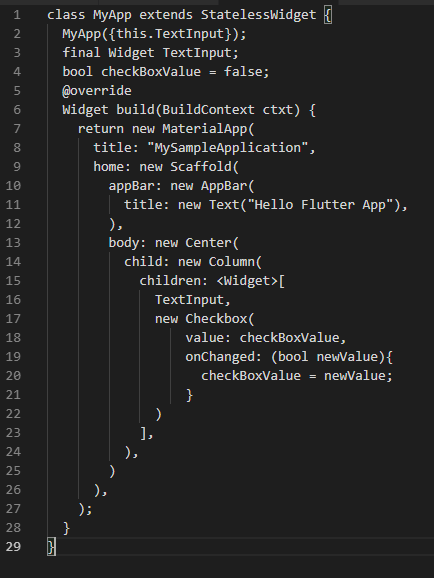
\includegraphics[width=75mm, height=75mm,scale=0.5]{img/stateless.PNG}
\caption{Code sample for stateless widget}
\label{fig:stateless}
\end{figure}

\subsubsection{Stateful widget}
Stateful widgets are dynamic or has a mutable state.Stateful widgets are widgets which can be read synchronously, when it is created and may change over the lifetime of the widget. The state can be reloaded by called the setState() method. In order to create a Stateful widget two classes must be made. One of which is created by extending statefulwidget(called myApp) and and another is created by entending the generic state<myApp>(this class is called myAppState). The typical hierarchy structure of a Stateful widget is matericalApp/home/scaffold/body/center/row/column/checkbox.\cite{widgets} \cite{stateful} Stateful widgets idea was originally taken from react native. Eg. the state can not  be change outside of the state. A real example as to when a stateful widget is used is when having a button on a page such as a like button in order to keep track of how many times this button is pressed by the user the button must be located within a Stateful widget class. \cite{choudhary_2019}


\begin{figure}[ht!]
    \centering
 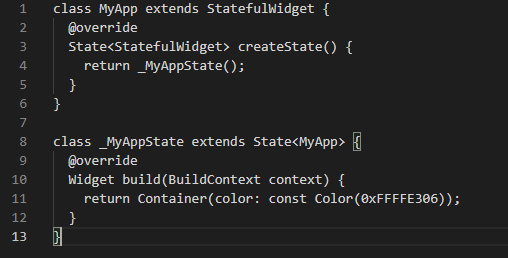
\includegraphics[width=75mm, height=75mm,scale=0.5]{img/stateful.PNG}
\caption{Code sample for stateful widget}
\label{fig:stateful}
\end{figure}

\subsubsection{inherited widgets}
An inherited widget is needed when the widget heirarchy gets very large and and information needs to be passed or accessed from a lower branch of the hierachy. A inheritied widget is a widget that can get called directly from any wiget in the tree structure below it.Inherited widgets are ideally kept small for good coding practise.\cite{fidanboylu_2019}.Theme is a type of inherited widget. It can be used in the context theme.of(context).primaryColor. This gets the global theme of a material app. An inheritied widget is not able to be changed over time.Similar to stateless widgets they can only be replaced by rebuilding the entire widget.\cite{inherited_widgets}

\subsubsection{Keys}
A key in flutter is an identifier for widgets and elements. These are rarely used but when used they are ideal for preserving a scroll location and keeping the state when modifying a collection or database.\cite{key_widgets}A to do list application is an example of a time that a key would be useful.Adding, updating, removing and creating items in a collection. Keys are only nessary if the entire subtree is stateless. Keys enable the item to be stateful and ables the subtree to keep track of the items state when the widget is reloaded. \cite{keys}

\subsection{Advantages of Flutter}

\subsubsection{Fast Code Development}
Flutter offers a Fast Code Development rate this is due to the fact that it is a single code base for both android and ISO development.This is known as a cross platform framework.All applications developed in flutter are 2D. Flutter also offers a "hot reload" this enables users to work with developers and easily see changes been made. This hot reload is done in the command prompt which the application is running. Hot reload works by injecting updated source code into the running application on the dart virtual machine.\cite{faq_2019}
\subsubsection{Open Source}
Flutter is an open source framework.It is created by google and has a large community which means the documentation is extensive and the language of dart is becoming more popular. Flutter has numerous build in API's to support use of camera, geolocation,network storage and more.\cite{pros_cons}
\subsubsection{Less Code}
There is less code to write when using flutter. Flutter is programmed in Dart. This is a object oriented programming language. Dart has similarities to React-native because its programming style is reactive and declarative.\cite{pros_cons} Reactive coding ensures only having to declare something once in the code base. This ensures that there is less code to write along with the fact that is becomes more readable and reusable.\cite{depth_flutter_2019}
\subsubsection{Model View Presenter (MVP)}
Flutter is ideal for MVP(model, view, presenter) pattern. The MVP is replacing the MVC, the controlled is exchanged for the presenter. This is idea because it enables the devloper to create an application to show the customers very fast on both iso and android on one code base saving time.\cite{pros_cons}.

\subsection{Disadvantages of Flutter}

\subsubsection{Mobile Developement alone}
Flutter caters to mobile Development alone.(andriod and Ios). Flutter is unable to create web applications, This is a limitation and may be a reason a company would opt against flutter.

\subsubsection{Lack Third party libraries}
Flutter is limited to the amount of third party libraries available to it. This is due to the fact that it is relatively new on the market and is based on dart.\cite{pros_cons} React-native has fully extensive third party libraries. It is based on JavaScript so therefore there were already libraries it could use before created.Dart was created by google also. Therefore it has not developed much external libraries. However these libraries are extending every day.Flutter takes care of User Interface packages needs with widgets. Long term development can be limited.\cite{good_bad}

\subsubsection{Large File Size}
Flutters application size is much larger then native applications. The original hello world in flutter was 6.7mb. After much complaints from developers, the flutter team managed to reduce the size to 4.7mb. At this the simple hello world application is still very large in comparison to java at 539kb and kotlin at 550kb.\cite{faq_2019} \cite{good_bad}



\chapter{Methodology}
\section{Project Management}

Project Management is a key element of any task to ensure that the project was laid out correctly and each component part is complete at a given date etc. Because this project was completed by a team it was important both members completed each task. In order to track the project a gantt chart was used. This broke down each step of the project and the expected time limits for each section.

\subsection{Agile}

The project used Agile project management methodologies.An iterative approach was taken. This meant that each week certain tasks are completed. The project team meet 3 times a week to discuss what has been completed since the last meeting, what has to be completed before the next and discuss any  difficulties experienced thought out the duration. The meetings are short and concise. Once a week the team met their mentor and explained what was completed since the last meeting and is to be done before the next. These weekly meetings were the iterative approach. Each week the process would be repeated to meet, plan, design, develop, test and evaluate.

\begin{figure}[ht!]
    \centering
 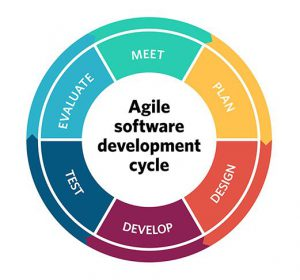
\includegraphics[width=75mm, height=75mm,scale=0.5]{img/agile.jpg}
\caption{Agile Life Cycle}
\label{fig:agile}
\end{figure}

\subsubsection{Breakdown of agile}
During the meeting and planning phase. The milestones for the project were identified and broken down into simpler, more manageable tasks. The tasks are then grouped into sprints lasting one week each. These are the tasks to be complete before each meeting. Each sprint started after the weekly meeting with the supervisor and terminated before the next weeks meeting. After each sprint before the meeting phase a review was carried out on the tasks completed in the last sprint. If there were changed to make these were completed in the next sprint. Testing is completed after every 2/3 weeks in the form of unit tests and widget tests.\cite{Agile}

\begin{figure}[ht]
    \centering
 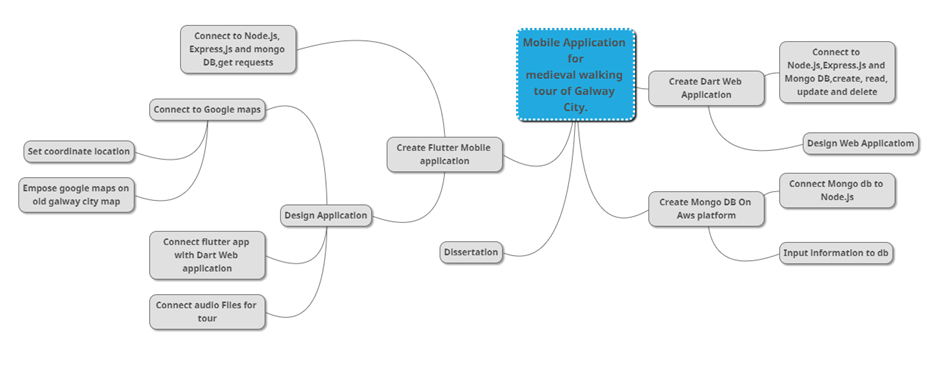
\includegraphics[width=135mm, height=50mm,scale=0.5]{img/plan.png}
\caption{Agile Life Cycle}
\label{fig:Project Plan}
\end{figure}

\subsection{Managing Project}
In order to manage this project GitHub was used. This was very useful due to it being a team project. It enables both members of the team to work on separate individual branches. After each iteration these branches were merged int the master branch. After each integration the project was at a working state of the project. This could be used for industry standard as continuous delivery. For this project is ment that after each sprint there was a working version to present to customer and supervisor. Although it is a working version is may still need changes in the next sprint.At the beginning of each sprint all branches pull from the master so as every team member is working of the same code.
\section{System Architecture}
\section{Technologies}
\subsection{Server}
\subsection{Client}
\section{System Integration}
Due to this project being produced in conjunction with Galway Civic trust,working closely with Michael Quinn to produce the exact item he wishes to publish is necessary. In order to do this Software engineering techniques are being used to ensure the customer receives exactly whats needed. The main approaches used are test driven development(TDD), behaviour driven development(BDD) and user storyboards.

\subsection{Storyboards}

Storyboards were used to allow the customer give the developers a high level view of expected design of the application. This is done using a blank page and the customer draws a simple representation of what they want to application to look like. This gives the developers a better understanding and idea what needs to be done and can help break down upcoming tasks to be completed. The storyboard used is taken from the agile methodology and is continuously being referred to and brought to each meeting with the customer to ensure every design requirement is clearly met. \cite{StoryBoard}

\subsection{Behaviour Driven Development}

Behaviour driven development is another agile software development methodology. It is designed base what the user wants and how the user explains what the visual display of the application should be. The customer/user gives a list of behaviours they wish the application the be able to accomplish. These simple requests and made into a task or multiple tasks for the developer. When the application is complete the original requirements are made into unit tests.\cite{BDD} 

\subsection{Test Driven Development}

Test Driven Development is based predominantly on unit testing. However they are very different because test driven development is when the unit tests are written before the code has been created. This means the developers are using the unit tests as a guild and the tests alone break down the overall task needing to be completed.The tests will initially fail and the developers write minimal code in order the the tests to pass. This is process in continuously repeated in order for the application to pass each test. These tests are commonly automated.\cite{TDD}

\chapter{Results}
\section{Results of the Application}
\section{Testing}
Testing is an essential part of any software development life cycle. The importance of testing in software development life cycle is to improve reliability, performance and other important factors.\cite{TestingLifeCycle} Each component of the project can be tested individually.
 
\subsection{Unit Tests}

Unit tests are individual tests to check functions,methods or classes. A test library is imported into the flutter application. The developer/tester can run the unit tests from the terminal to check for success or failure. Unit tests can test that visual aspects of the application are working correctly along with connection to database.

\subsection{Widget Testing}

A widget test tests a single widget. Testing a widget involves multiple classes and requires a test environment that provides the appropriate widget life cycle context. \cite{testing}. It tests that the widget user interface performs as expected both visually and its interactions. A widget should be able to check for user input and check for responses for the user based on actions performed. It is similar to unit testing because it tests the environment and is usually created to test certain actions alone.

\subsection{Integration Testing}

Integration testing is used to test the flutter application in whole. This tests that each function checked in unit and widget tests also work when Incorporated with the remainder of the application. Integration testing is also used to test the performance of the application. This was done to test that the application could retrieve information from the database by many users simultaneously. Developers/testers can run the command "flutter driver" which sets up the test harness, builds and installs the application and runs the integration tests on the application. \cite{IntegrationTest}

\subsection{Fuzz Testing}
In order to carry out tests on the web application and mongo database, fuzz testing is used. This means testing the architecture by giving it a large variety of inputs. The web application updated, creates and deletes inputs from the mongo db. The input size is limited and this limit is tested to the max though fuzz tests, along with invalid inputs such as no input and numeric input alone. This testing is to be completed after the basic level of testing.

\begin{figure}[ht!]
    \centering
 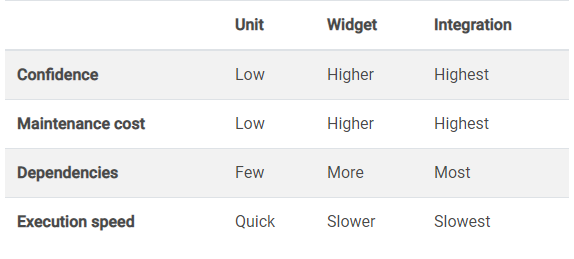
\includegraphics[width=125mm,scale=0.5]{img/Capture.PNG}
\caption{Testing:Types of testing}
\cite{testing}
\label{fig:method}
\end{figure}

\chapter{Conclusion}

 






 


